% !TeX spellcheck = en

\documentclass[german]{beamer}
%\documentclass[aspectratio=169]{beamer}
\everymath{\displaystyle}
%\usepackage{amsmath}
%\usepackage{amssymb}
\usepackage{rotating}
\usepackage{verbatim}
\usepackage{latexsym}
\usepackage{graphicx}
\usepackage{tabularx}
\usepackage{ragged2e}
%\usepackage{eurosym}   % Euro symbol: \euro
\usepackage{listings}
\usepackage{multirow}
\usepackage{colortbl}
\usepackage{textcomp}  % many special symbols
\usepackage{lmodern}
\usepackage{times}
\usepackage[T1]{fontenc}
\usepackage[utf8]{inputenc}
\usepackage[german]{babel}
\usepackage{booktabs}
\usepackage{caption}
\usepackage{svg}
\captionsetup[figure]{labelformat=empty}
\usepackage[nodayofweek,level]{datetime}
\usepackage{subcaption}
\usepackage{marvosym}
\usepackage{wasysym}
\usepackage{xcolor,colortbl}
\definecolor{lightblue}{rgb}{0.68, 0.85, 0.9}

\newcommand{\code}[1]{{\fontfamily{txtt}\selectfont#1}} % code-like font
\newcolumntype{\XL}[1]{>{\hsize=#1\hsize\raggedright\arraybackslash}X}% left aligned tabularx column, which takes as a parameter the width respective to X

\usepackage[binary-units=true, output-decimal-marker={.}]{siunitx} % Required for \SI commands
\usepackage{tikz}
\usetikzlibrary{shapes,backgrounds}
\tikzset{>=latex}

\graphicspath{{./images/}}
\PassOptionsToPackage{demo}{graphicx}
\newcommand{\credit}[1]{\par \scriptsize \itshape#1}

\usetheme[fb2]{FrankfurtUniversity}

\defbeamertemplate{subsection page}{mine}[1][]{%
  \begin{centering}
    {\usebeamerfont{subsection name}\usebeamercolor[fg]{subsection name}#1}
    \vskip1em\par
    \begin{beamercolorbox}[sep=8pt,center,#1]{part title}
      \usebeamerfont{subsection title}\insertsubsection\par
    \end{beamercolorbox}
  \end{centering}
}

\setbeamercovered{invisible}
\setbeamertemplate{blocks}[rounded][shadow=false]

\setbeamertemplate{bibliography item}[text] % Wegen den Nummern an den Referenzen !!!

\newcommand{\myEmail}{cocos@fb2.fra-uas.de}
\newcommand{\myTitle}{TITLE}
\newcommand{\mySubtitle}{Subtitle}
\newcommand{\myAuthorOne}{Henry-Norbert Cocos}

\newcommand{\thisInstitute}{Frankfurt University of Applied Sciences}
\newcommand{\thisFacultyGerman}{Fachbereich 2 - Informatik und Ingenieurwissenschaft}
\newcommand{\thisCityGerman}{60318 Frankfurt am Main}
\newcommand{\thisStudyGerman}{Informatik}
\newcommand{\thisFacultyEnglish}{Department of Computer Science and Engineering}
\newcommand{\thisStudyEnglish}{Computer Science}
\newcommand{\thisCityEnglish}{D-60318 Frankfurt am Main}


\newif\ifgerman
\germantrue % wenn auskommentiert = englisch

\title{\myTitle}
\subtitle{\footnotesize\mySubtitle}
\author{\myAuthorOne}

\author{\myAuthorOne}

\institute{
	\nolinkurl{\myEmail}\\

	\ifgerman
	\textbf{\thisStudyGerman}\newline
	\textbf{\thisFacultyGerman}\newline
	\textbf{\thisInstitute}\newline
	\textbf{\thisCityGerman}
	\else
	\textbf{\thisStudyEnglish}\newline
	\textbf{\thisFacultyEnglish}\newline
	\textbf{\thisInstitute}\newline
	\textbf{\thisCityEnglish}
	\fi	
}


\date{\today}

% Informationen für PDF-Dokument
\hypersetup{
	pdfpagemode={UseOutlines},
	bookmarksopen=true,
	bookmarksopenlevel=0,
	hypertexnames=false,
	colorlinks=true,% Set to false to disable coloring links
	citecolor=black,% The color of citations Für PDF=magenta Für Druck=black
	linkcolor=black,% The color of references to document elements (sections, figures, etc) Für PDF=mdtBlue Für Druck=black
	urlcolor=black,% The color of hyperlinks (URLs) Für PDF=mdtBlue Für Druck=black
	pdfstartview={FitV},
	unicode,
	breaklinks=true,
	pdftitle={\myTitle},
	pdfsubject={\mySubtitle},
	pdfauthor={\myAuthorOne},
	pdfkeywords={\myTitle,}
}

\begin{document}

\begin{frame}
\titlepage
\end{frame}
%\addtocounter{framenumber}{-2}

\begin{frame}{{\ifgerman Inhalt\else Content\fi}}
	\tableofcontents
\end{frame}

\AtBeginSection[]
{
	\ifgerman
	\begin{frame}<beamer>{{\ifgerman Inhalt\else Content\fi}}
		\tableofcontents[currentsection] %,currentsubsection] % only sections are displayed
	\end{frame}
}

%%%%%%%%%%%%%%%%%%%%%%%%%%%%%%%%%%%%%%%%%%%%%%%%%%%%%%%%%%%%%%%%%%%%%%%%%%%%%%%%%
% ALLE ABSCHNITTE
%%%%%%%%%%%%%%%%%%%%%%%%%%%%%%%%%%%%%%%%%%%%%%%%%%%%%%%%%%%%%%%%%%%%%%%%%%%%%%%%%%
% !TeX spellcheck = en

%%%%%%%%%%%%%%%%%%%%%%%%%%%%%%%%%%%%%%%%%%%%%%%%%%%%%%%%%%%%%%%%%%%%%%%%%%%%%%%%%%
% SECTION
%%%%%%%%%%%%%%%%%%%%%%%%%%%%%%%%%%%%%%%%%%%%%%%%%%%%%%%%%%%%%%%%%%%%%%%%%%%%%%%%%%	
\section{Grundlagen}

%%%%%%%%%%%%%%%%%%%%%%%%%%%%%%%%%%%%%%%%%%%%%%%%%%%%%%%%%%%%%%%%%%%%%%%%%%%%%%%%%%
% SUBSECTION
%%%%%%%%%%%%%%%%%%%%%%%%%%%%%%%%%%%%%%%%%%%%%%%%%%%%%%%%%%%%%%%%%%%%%%%%%%%%%%%%%%	
\subsection{README}


%%%%%%%%%%%%%%%%%%%%%%%%%%%%%%%%%%%%%%%%%%%%%%%%%%%%%%%%%%%%%%%%%%%%%%%%%%%%%%%%%%
% FRAME
%%%%%%%%%%%%%%%%%%%%%%%%%%%%%%%%%%%%%%%%%%%%%%%%%%%%%%%%%%%%%%%%%%%%%%%%%%%%%%%%%%
\begin{frame}[fragile]
	% [fragile] braucht man, wenn man \verb oder \verbatim auf der Folie verwendet!
	\frametitle{README}
	\begin{itemize}
		\item Das hier ist die Folienvorlage zum Kurs \textbf{Betriebssysteme und Rechnernetze}.
		\item Diese Vorlage soll den Einstieg erleichtern.
		\item Wird unter Linux im Verzeichnis mit der Quelldatei (\texttt{.tex}) das Kommando \texttt{make} eingegeben, wird eine PDF- und eine PS-Datei erzeugt. Beide haben den gleichen Inhalt.
		\item Ein aktuelles \LaTeX\ sollte installiert sein.
		\item Zum Editieren kann ein Texteditor (bspw. Kate) oder eine IDE wie bspw. TeXStudio \cite{TeXStudio} verwendet werden.
		\item Wer unter Windows die Folien machen möchte, dem empfehle ich MiK\TeX\footnote{\texttt{http://www.miktex.org}} \cite{MikTeX} und \TeX nicCenter\footnote{\texttt{http://www.texniccenter.org}} \cite{TexNic}. Hierzu habe ich aber keine Erfahrungswerte.
	\end{itemize}
\end{frame}

\begin{frame}[fragile]
	\frametitle{\LaTeX Beamer}
	\begin{itemize}
		\item Diese Vorlage nutzt die \LaTeX-Klasse \texttt{beamer}.
		\item Eine gute Dokumentation über diese Klasse befindet sich hier:\\
		\url{http://www2.informatik.hu-berlin.de/~mischulz/beamer.html}
		\item Diese Quelle ist auch hilfreich:\\
		\url{http://www.physik.uni-freiburg.de/~tooleh/latex_beamerkurs.pdf}
		\item Google findet sehr viele hilfreiche Links zum Thema \textbf{LaTeX Beamer}.
	\end{itemize}
\end{frame}


%%%%%%%%%%%%%%%%%%%%%%%%%%%%%%%%%%%%%%%%%%%%%%%%%%%%%%%%%%%%%%%%%%%%%%%%%%%%%%%%%%
% SECTION
%%%%%%%%%%%%%%%%%%%%%%%%%%%%%%%%%%%%%%%%%%%%%%%%%%%%%%%%%%%%%%%%%%%%%%%%%%%%%%%%%%	
\section{Textformatierung}

%%%%%%%%%%%%%%%%%%%%%%%%%%%%%%%%%%%%%%%%%%%%%%%%%%%%%%%%%%%%%%%%%%%%%%%%%%%%%%%%%%
% SUBSECTION
%%%%%%%%%%%%%%%%%%%%%%%%%%%%%%%%%%%%%%%%%%%%%%%%%%%%%%%%%%%%%%%%%%%%%%%%%%%%%%%%%%	
\subsection{Schriften und Sonderzeichen}


%%%%%%%%%%%%%%%%%%%%%%%%%%%%%%%%%%%%%%%%%%%%%%%%%%%%%%%%%%%%%%%%%%%%%%%%%%%%%%%%%%
% FRAME
%%%%%%%%%%%%%%%%%%%%%%%%%%%%%%%%%%%%%%%%%%%%%%%%%%%%%%%%%%%%%%%%%%%%%%%%%%%%%%%%%%
\begin{frame}[fragile]
	\frametitle{Schriften und Sonderzeichen}
	\begin{itemize}
		\item Es gibt verschiedene Schriftsätze: \textbf{Bold Face}, \textrm{Roman}, \textit{Italic}, \texttt{Typewriter}, \textsf{Sans Serif}, \textsl{Slanted}, \textsc{Small Caps}.
		\item \textcolor{blue}{Farben} sollte man \textcolor{red}{nicht} zu viel einsetzen.
		\item Ein paar Sonderzeichen: \textbackslash, \$, \&, \euro, \%, \#, \textunderscore, \textasciitilde, \textasciicircum, \textbar, \{, \}
		\item Weitere Sonderzeichen: \copyright, \textregistered, \texttrademark, \S, \P, \pounds, \dag, \ddag, \textbullet
		\item Fortsetzungspunkte macht das Kommando \verb!\dots!. Ergebnis: \dots
	\end{itemize}
\end{frame}

%%%%%%%%%%%%%%%%%%%%%%%%%%%%%%%%%%%%%%%%%%%%%%%%%%%%%%%%%%%%%%%%%%%%%%%%%%%%%%%%%%
% SUBSECTION
%%%%%%%%%%%%%%%%%%%%%%%%%%%%%%%%%%%%%%%%%%%%%%%%%%%%%%%%%%%%%%%%%%%%%%%%%%%%%%%%%%	
\subsection{Schriftgrößen}


%%%%%%%%%%%%%%%%%%%%%%%%%%%%%%%%%%%%%%%%%%%%%%%%%%%%%%%%%%%%%%%%%%%%%%%%%%%%%%%%%%
% FRAME
%%%%%%%%%%%%%%%%%%%%%%%%%%%%%%%%%%%%%%%%%%%%%%%%%%%%%%%%%%%%%%%%%%%%%%%%%%%%%%%%%%
\begin{frame}[fragile]
	\frametitle{Schriftgrößen}
	
	\Huge
	\verb!\Huge!
	\normalsize
	
	\huge
	\verb!\huge!
	\normalsize
	
	\LARGE
	\verb!\LARGE!
	\normalsize
	
	\Large
	\verb!\Large!
	\normalsize
	
	\large
	\verb!\large!
	\normalsize
	
	\normalsize
	\verb!\normalsize!
	\normalsize
	
	\small%%%%%%%%%%%%%%%%%%%%%%%%%%%%%%%%%%%%%%%%%%%%%%%%%%%%%%%%%%%%%%%%%%%%%%%%%%%%%%%%%%
	% FRAME
	%%%%%%%%%%%%%%%%%%%%%%%%%%%%%%%%%%%%%%%%%%%%%%%%%%%%%%%%%%%%%%%%%%%%%%%%%%%%%%%%%%
	\verb!\small!
	\normalsize
	
	\footnotesize
	\verb!\footnotesize!
	\normalsize
	
	\scriptsize
	\verb!\scriptsize!
	\normalsize
	
	\tiny
	\verb!\tiny!
	\normalsize
\end{frame}


%%%%%%%%%%%%%%%%%%%%%%%%%%%%%%%%%%%%%%%%%%%%%%%%%%%%%%%%%%%%%%%%%%%%%%%%%%%%%%%%%%
% SUBSECTION
%%%%%%%%%%%%%%%%%%%%%%%%%%%%%%%%%%%%%%%%%%%%%%%%%%%%%%%%%%%%%%%%%%%%%%%%%%%%%%%%%%	
\subsection{Blöcke}


%%%%%%%%%%%%%%%%%%%%%%%%%%%%%%%%%%%%%%%%%%%%%%%%%%%%%%%%%%%%%%%%%%%%%%%%%%%%%%%%%%
% FRAME
%%%%%%%%%%%%%%%%%%%%%%%%%%%%%%%%%%%%%%%%%%%%%%%%%%%%%%%%%%%%%%%%%%%%%%%%%%%%%%%%%%
\begin{frame}[t]
	% [t] legt fest, dass der Text oben auf der Folie platziert wird.
	\frametitle{Blöcke}
	\begin{itemize}
		\item Es gibt verschiedene Arten von Blöcken:
	\end{itemize}
	\begin{block}{Blocktitel}
		Blocktext
	\end{block}
	
	\begin{exampleblock}{Blocktitel}
		Blocktext
	\end{exampleblock}
	
	\begin{alertblock}{Blocktitel}
		Blocktext
	\end{alertblock}
\end{frame}


%%%%%%%%%%%%%%%%%%%%%%%%%%%%%%%%%%%%%%%%%%%%%%%%%%%%%%%%%%%%%%%%%%%%%%%%%%%%%%%%%%
% SUBSECTION
%%%%%%%%%%%%%%%%%%%%%%%%%%%%%%%%%%%%%%%%%%%%%%%%%%%%%%%%%%%%%%%%%%%%%%%%%%%%%%%%%%	
\subsection{Bilder}


%%%%%%%%%%%%%%%%%%%%%%%%%%%%%%%%%%%%%%%%%%%%%%%%%%%%%%%%%%%%%%%%%%%%%%%%%%%%%%%%%%
% FRAME
%%%%%%%%%%%%%%%%%%%%%%%%%%%%%%%%%%%%%%%%%%%%%%%%%%%%%%%%%%%%%%%%%%%%%%%%%%%%%%%%%%
\begin{frame}
	% [t] legt fest, dass der Text oben auf der Folie platziert wird.
	\frametitle{Bilder}
	\begin{itemize}
		\item Hier ist ein Bild:
	\end{itemize}
	\begin{center}
		
\includegraphics[height=4cm]{Pinguin.pdf}
		% Die Dateiendung muss man nicht angeben.
		% Man hätte auch alternativ die Breite mit "width" angeben können.
	\end{center}
	\begin{itemize}
		\item Bilder sollten im Format Encapsulated PostScript (\texttt{.eps}) sein. Dieses Dateiformat kann man mit Gimp und vielen anderen Programmen erzeugen.
	\end{itemize}
\end{frame}


%%%%%%%%%%%%%%%%%%%%%%%%%%%%%%%%%%%%%%%%%%%%%%%%%%%%%%%%%%%%%%%%%%%%%%%%%%%%%%%%%%
% SUBSECTION
%%%%%%%%%%%%%%%%%%%%%%%%%%%%%%%%%%%%%%%%%%%%%%%%%%%%%%%%%%%%%%%%%%%%%%%%%%%%%%%%%%	
\subsection{Tabellen}


%%%%%%%%%%%%%%%%%%%%%%%%%%%%%%%%%%%%%%%%%%%%%%%%%%%%%%%%%%%%%%%%%%%%%%%%%%%%%%%%%%
% FRAME
%%%%%%%%%%%%%%%%%%%%%%%%%%%%%%%%%%%%%%%%%%%%%%%%%%%%%%%%%%%%%%%%%%%%%%%%%%%%%%%%%%
\begin{frame}[fragile]
	\frametitle{Tabellen}
	\begin{itemize}
		\item Es gibt mehrere Umgebungen, um Tabellen zu machen. \texttt{tabular} ist nur eine von vielen.
	\end{itemize}
	
	\begin{center}
		\begin{tabular}{|c|l|c|r|}
			\hline
			\textbf{Zeile} & \textbf{Linksbündig} & \textbf{Zentriert} & \textbf{Rechtsbündig} \\
			\hline\hline
			1 & Zeile 1 & Zeile 1 & Zeile 1 \\
			2 & Zeile 2 & Zeile 2 & Zeile 2 \\
			3 & Zeile 3 & Zeile 3 & Zeile 3 \\
			\hline
		\end{tabular}
	\end{center}
	
	\begin{itemize}
		\item Das geht natürlich auch ohne die Rahmen:
	\end{itemize}
	
	\begin{center}
		\begin{tabular}{clcr}
			\textbf{Zeile} & \textbf{Linksbündig} & \textbf{Zentriert} & \textbf{Rechtsbündig} \\
			1 & Zeile 1 & Zeile 1 & Zeile 1 \\
			2 & Zeile 2 & Zeile 2 & Zeile 2 \\
			3 & Zeile 3 & Zeile 3 & Zeile 3 \\
		\end{tabular}
	\end{center}
\end{frame}


%%%%%%%%%%%%%%%%%%%%%%%%%%%%%%%%%%%%%%%%%%%%%%%%%%%%%%%%%%%%%%%%%%%%%%%%%%%%%%%%%%
% SUBSECTION
%%%%%%%%%%%%%%%%%%%%%%%%%%%%%%%%%%%%%%%%%%%%%%%%%%%%%%%%%%%%%%%%%%%%%%%%%%%%%%%%%%	
\subsection{Mehrspaltige Folien}


%%%%%%%%%%%%%%%%%%%%%%%%%%%%%%%%%%%%%%%%%%%%%%%%%%%%%%%%%%%%%%%%%%%%%%%%%%%%%%%%%%
% FRAME
%%%%%%%%%%%%%%%%%%%%%%%%%%%%%%%%%%%%%%%%%%%%%%%%%%%%%%%%%%%%%%%%%%%%%%%%%%%%%%%%%%
\begin{frame}
	\frametitle{Mehrspaltige Folien}
	\begin{columns}
		\column{.45\textwidth}
		Mehrspaltige Folien können einfach mit \texttt{columns} realisiert werden.
		\column{.45\textwidth}
		\begin{enumerate}
			\item Ein Eintrag
			\item Noch ein Eintrag
		\end{enumerate}
	\end{columns}
\end{frame}

%%%%%%%%%%%%%%%%%%%%%%%%%%%%%%%%%%%%%%%%%%%%%%%%%%%%%%%%%%%%%%%%%%%%%%%%%%%%%%%%%%
% SUBSECTION
%%%%%%%%%%%%%%%%%%%%%%%%%%%%%%%%%%%%%%%%%%%%%%%%%%%%%%%%%%%%%%%%%%%%%%%%%%%%%%%%%%	
\subsection{Zitieren und Quellenangaben}


%%%%%%%%%%%%%%%%%%%%%%%%%%%%%%%%%%%%%%%%%%%%%%%%%%%%%%%%%%%%%%%%%%%%%%%%%%%%%%%%%%
% FRAME
%%%%%%%%%%%%%%%%%%%%%%%%%%%%%%%%%%%%%%%%%%%%%%%%%%%%%%%%%%%%%%%%%%%%%%%%%%%%%%%%%%
\begin{frame}[fragile]
	\frametitle{Ziteren und Quellenangaben}
	
	\begin{itemize}
		\item Quellen können im Text mit \verb|\cite| gefolgt von einem Schlüssel gefolgt werden
		\item Beispielsweise produziert das Kommando\\ \verb|\cite{BibliographyLaTeX}|
		 die Referenz $\rightarrow$ \cite{BibliographyLaTeX}
		 \item Die Quellen werden in einer separaten \texttt{.bib} Datei angelegt
	\end{itemize}
	
\end{frame}		


%%%%%%%%%%%%%%%%%%%%%%%%%%%%%%%%%%%%%%%%%%%%%%%%%%%%%%%%%%%%%%%%%%%%%%%%%%%%%%%%%%
% ABSCHLUSS FRAME
%%%%%%%%%%%%%%%%%%%%%%%%%%%%%%%%%%%%%%%%%%%%%%%%%%%%%%%%%%%%%%%%%%%%%%%%%%%%%%%%%%
\ifgerman
\begin{frame}
	
	\begin{center}
		{\fontsize{30}{40}\selectfont Vielen Dank\\ für Ihre Aufmerksamkeit!}
	\end{center}
	%\vspace{12pt}
	\hfill
	
	\centering	
	\begin{minipage}{0.5\textwidth}
		\raggedright
		\textbf{Henry-Norbert Cocos, M.Sc}\\\vfill
		Frankfurt University of Applied Sciences\\\vfill
		Raum 1-230\\\vfill
		\phone~069 1533-2699\\\vfill
		\Letter~\nolinkurl{cocos@fb2.fra-uas.de}
		\Mundus~\url{www.henrycocos.de}
		\begin{figure}[htbp]
			\raggedright
			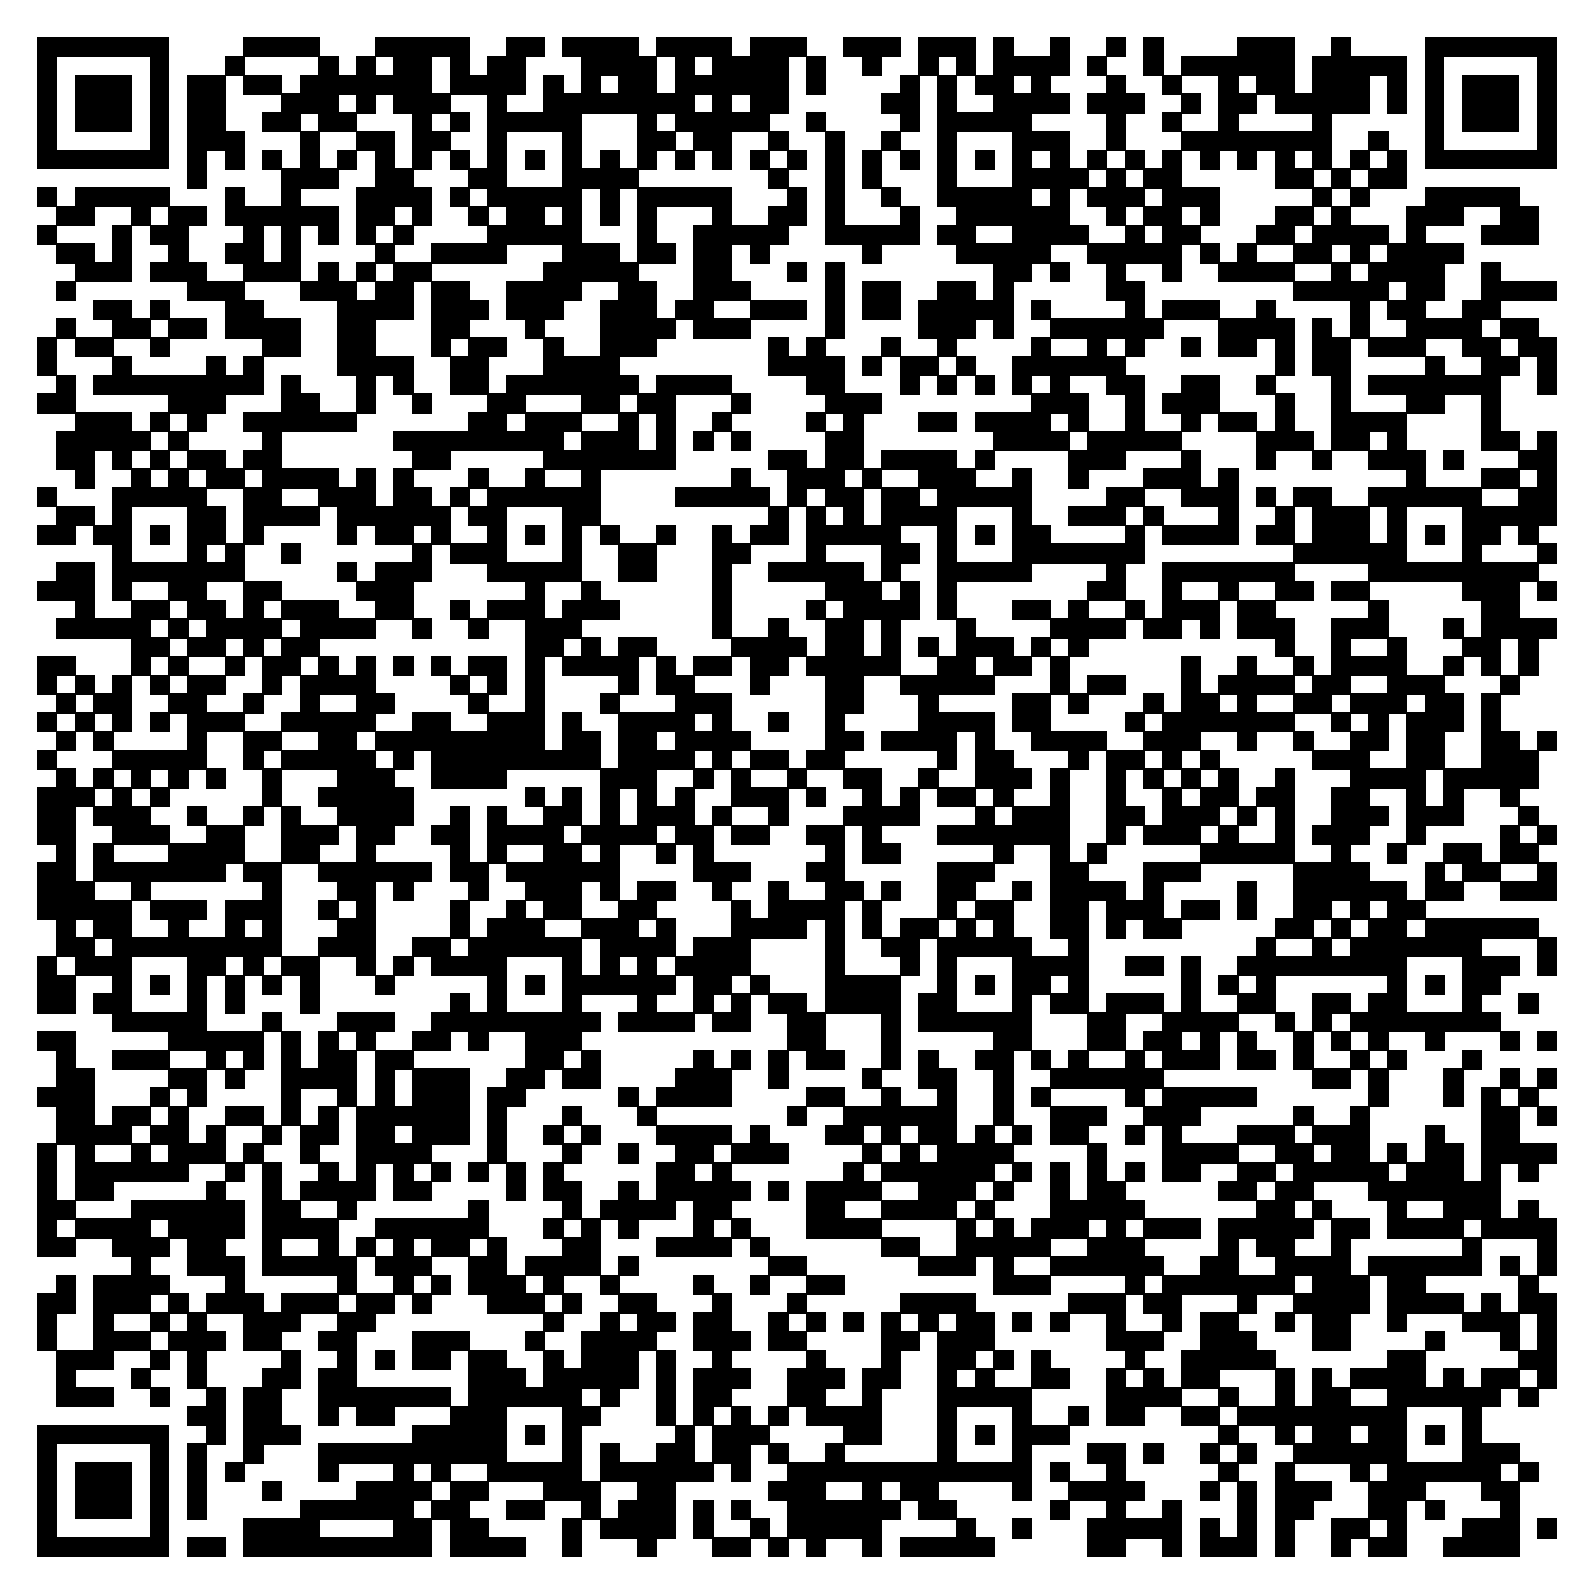
\includegraphics[width=0.25\textwidth]{Cocos_FRAUAS}
		\end{figure}
	\end{minipage}%
	\begin{minipage}{0.45\textwidth}
		\begin{figure}[htbp]
			\centering
			
\includegraphics[width=0.75\textwidth]{/logos/FRA-UAS_Logo}
		\end{figure}
		\vspace{40pt}
	\end{minipage}
\end{frame}

\else
%%%%%%%%%%%%%%%%%%%%%%%%%%%%%%%%%%%%%%%%%%%%%%%%%%%%%%%%%%%%%%%%%%%%%%%%%%%%%%%%%%
% FRAME
%%%%%%%%%%%%%%%%%%%%%%%%%%%%%%%%%%%%%%%%%%%%%%%%%%%%%%%%%%%%%%%%%%%%%%%%%%%%%%%%%%
\begin{frame}{}
	
	\begin{center}
		{\fontsize{30}{40}\selectfont Thank You\\ For Your Attention!}
	\end{center}
	%\vspace{12pt}
	\hfill
	
	\centering	
	\begin{minipage}{0.5\textwidth}
		\raggedright
		\textbf{Henry-Norbert Cocos, M.Sc}\\\vfill
		Frankfurt University of Applied Sciences\\\vfill
		Room 1-230\\\vfill
		\phone~+49 69 1533-2699\\\vfill
		\Letter~\nolinkurl{cocos@fb2.fra-uas.de}
		\Mundus~\url{www.henrycocos.de}
		\begin{figure}[htbp]
			\raggedright
			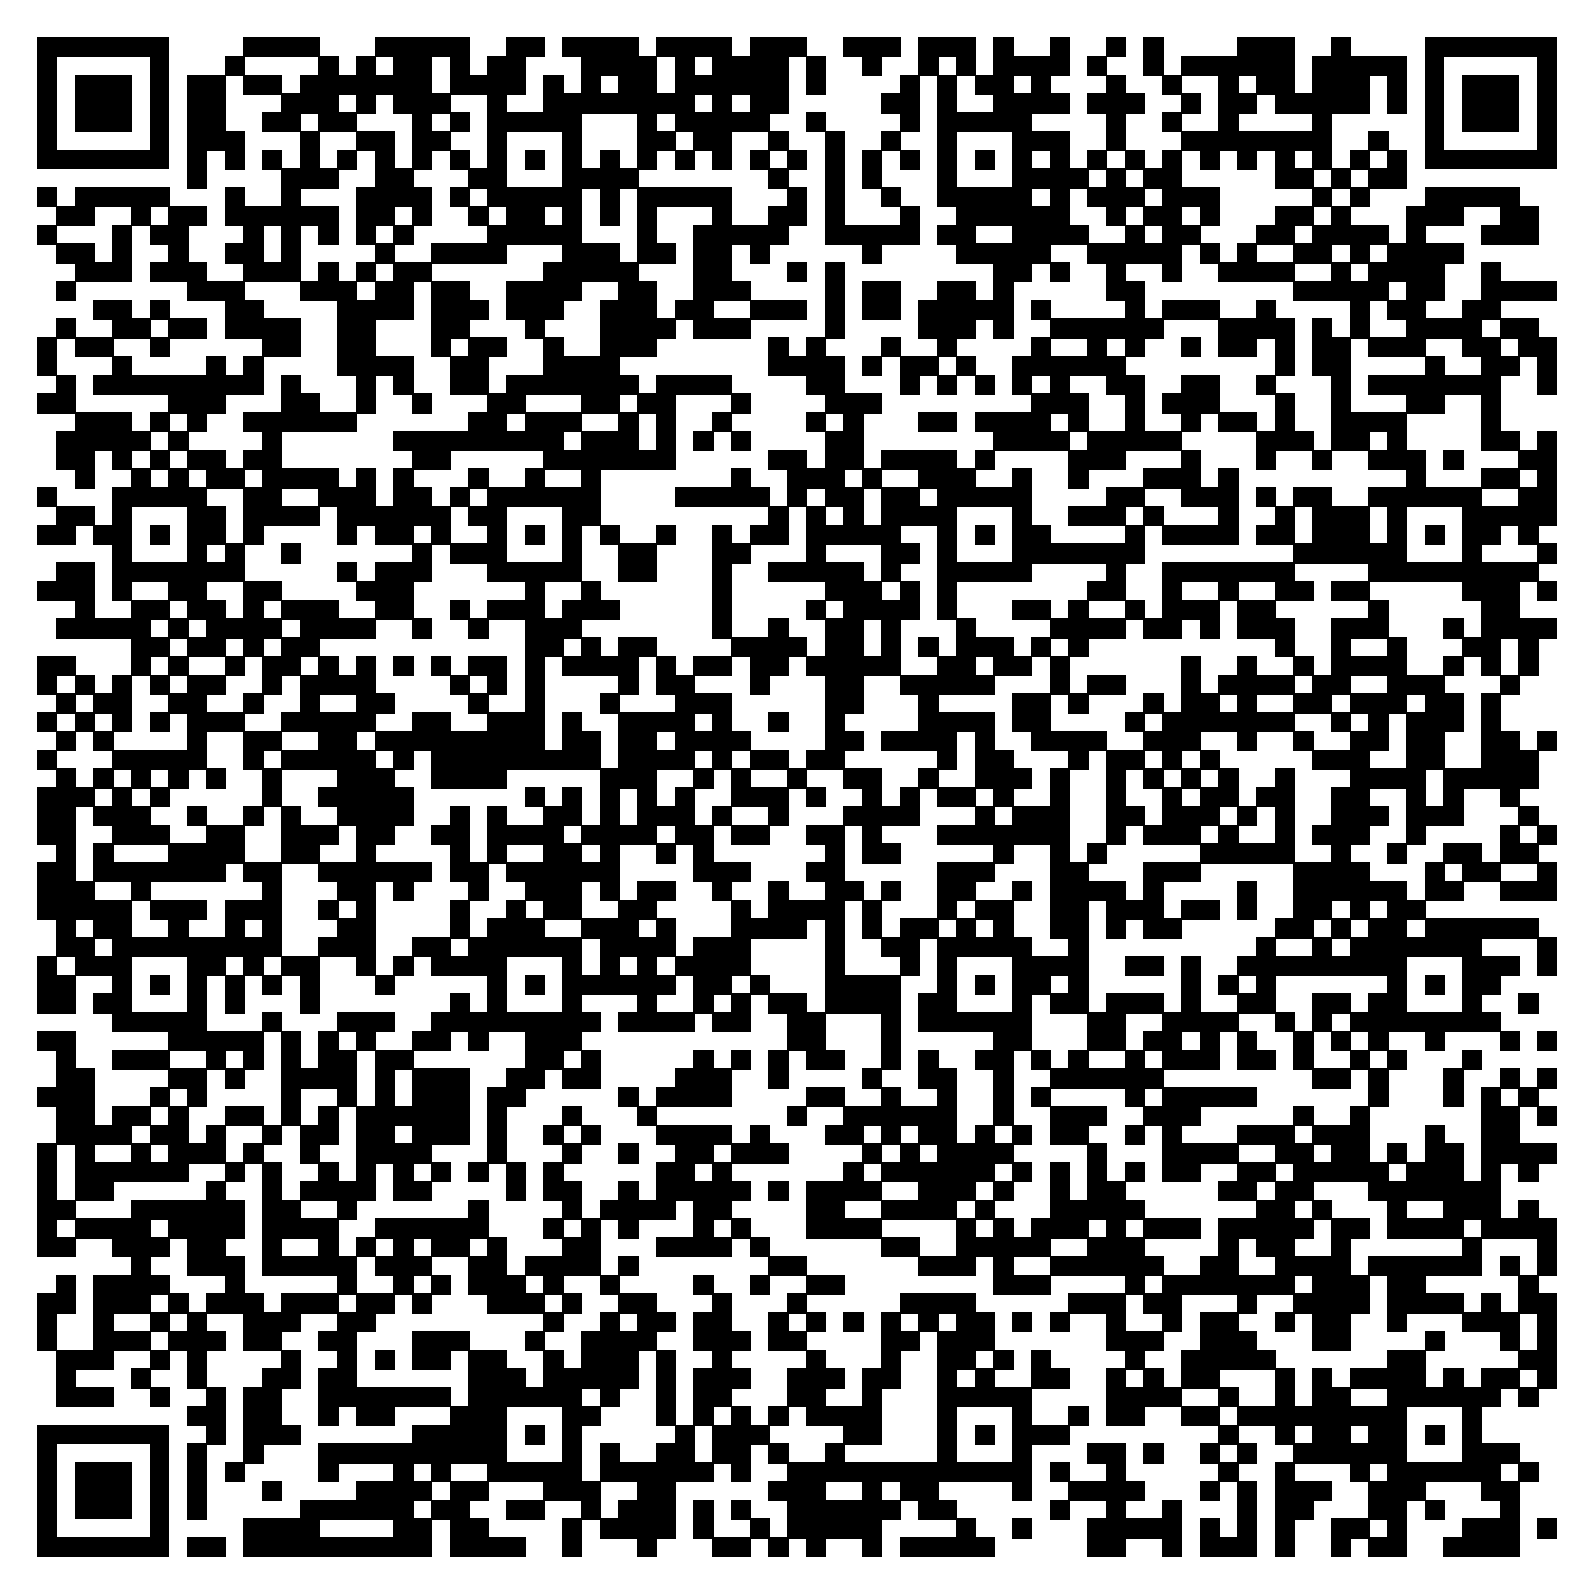
\includegraphics[width=0.25\textwidth]{Cocos_FRAUAS}
		\end{figure}
	\end{minipage}%
	\begin{minipage}{0.45\textwidth}
			\begin{figure}[htbp]
			\centering
			
\includegraphics[width=0.75\textwidth]{/logos/FRA-UAS_Logo}
		\end{figure}
		\vspace{40pt}
	\end{minipage}
	
\end{frame}
\fi


%%%%%%%%%%%%%%%%%%%%%%%%%%%%%%%%%%%%%%%%%%%%%%%%%%%%%%%%%%%%%%%%%%%%%%%%%%%%%%%%%%
% QUELLEN
%%%%%%%%%%%%%%%%%%%%%%%%%%%%%%%%%%%%%%%%%%%%%%%%%%%%%%%%%%%%%%%%%%%%%%%%%%%%%%%%%%
\ifgerman
\section{Quellen}
\label{sec:References}


\begin{frame}[plain,allowframebreaks]{Quellen}
	\small
	\bibliographystyle{IEEEtran}
	\bibliography{IEEEfull,references}
\end{frame}
\else
\section{References}
\label{sec:References}


\begin{frame}[plain,allowframebreaks]{References}
	\small
	\bibliographystyle{IEEEtran}
	\bibliography{IEEEfull,references}
\end{frame}
\fi

\end{document}